\documentclass[%
 reprint,
 amsmath,amssymb,
 aps,
 prb,
]{revtex4-2}

% ========================================
% Document Class and Package Setup
% ========================================
\usepackage{graphicx}
\usepackage{bm}

% Quantum mechanics notation
\usepackage{physics}

% Hyperlink configuration
\usepackage[colorlinks=true,
            linkcolor=blue,
            filecolor=blue,
            urlcolor=blue,
            citecolor=blue]{hyperref}

% Caption formatting
\usepackage{caption}
\captionsetup[figure]{
    justification=raggedright,
    labelfont={bf},
    name={Fig.},
    labelsep=period
}
\captionsetup[table]{
    labelfont={bf},
    name={Table},
    labelsep=period
}

% Equation numbering per section
\numberwithin{equation}{section}

% Typography tuning
\tolerance=1000
\emergencystretch=1em
\hyphenpenalty=3000
\exhyphenpenalty=3000
\flushbottom

% Microtypography
\usepackage[final]{microtype}

\usepackage{ragged2e}  % for \justifying command

% Table rules: \midrule, \addlinespace, \bottomrule
\usepackage{booktabs}

% Theorem environment
\usepackage{amsthm}
\newtheorem{theorem}{Theorem}[section]

% Code listings with syntax highlighting
\usepackage{listings}
\usepackage{xcolor}

% Color definitions (light blue palette for academic publication)
\definecolor{backcolour}{rgb}{0.96,0.97,0.98}
\definecolor{deepblue}{rgb}{0,0,0.5}
\definecolor{deepgreen}{rgb}{0,0.5,0.3}
\definecolor{deepgray}{rgb}{0.4,0.4,0.4}
\definecolor{stringcolor}{rgb}{0.2,0.4,0.6}

% Python listing style definition
\lstdefinestyle{pythonstyle}{
    backgroundcolor=\color{backcolour},
    commentstyle=\color{deepgreen}\itshape,
    keywordstyle=\color{deepblue}\bfseries,
    numberstyle=\tiny\color{deepgray},
    stringstyle=\color{stringcolor},
    basicstyle=\ttfamily\footnotesize,
    breakatwhitespace=false,
    breaklines=true,
    captionpos=b,
    keepspaces=true,
    numbers=left,
    numbersep=5pt,
    showspaces=false,
    showstringspaces=false,
    showtabs=false,
    tabsize=2,
    language=Python,
    frame=single,
    rulecolor=\color{deepgray}
}
\lstset{style=pythonstyle}

% Internal phase notation
\newcommand{\iphase}{\theta}  % internal geometric phase = ωt/2

% ========================================
% Document Begin
% ========================================
\begin{document}

% ========================================
% Title, Author, and Date
% ========================================
\title{Electron Interference from Internal Geometry: \\
Two-Kernel SU(2) Structure, Quartic Energy Flow, and an Intrinsic Visibility Limit}

\author{Satoshi Hanamura}
\email{hana.tensor@gmail.com}
\date{February 21, 2026}


\begin{abstract}
The electron is conventionally modeled as a point particle, with internal structure considered inaccessible or irrelevant to observable phenomena. This work explores an alternative geometric framework in which the electron possesses a minimal internal structure consisting of two energy kernels separated by the Compton wavelength. Energy circulates between these kernels through radiative exchange, giving rise to an internal geometric phase and a spinorial SU(2) structure. Observable interference patterns emerge from the quartic energy identity governing this internal circulation. When internal phases are not externally controlled, ensemble averaging yields a universal visibility bound of $\langle V \rangle = \sqrt{2}-1 \approx 0.4142$ for electron interference. Application of relativistic kinematics to the internal oscillatory motion leads to a characteristic velocity $v_{\mathrm{zb}} \simeq 0.04c$, derived from Lorentz contraction and the experimentally measured anomalous magnetic moment. This velocity represents a concrete prediction whose experimental verification or refutation would directly test the physical reality of internal Zitterbewegung dynamics.
\end{abstract}

\maketitle


% ========================================
% Section 1: Introduction
% ========================================
\section{Introduction}
\label{sec:introduction}

The interpretation of quantum mechanical phenomena has evolved considerably since the formulation of the Dirac equation, yet certain conceptual questions remain open. Among these is the physical status of Zitterbewegung---the rapid oscillatory motion predicted by relativistic wave equations. In standard treatments, this motion is often regarded as a formal feature arising from interference between positive- and negative-energy solutions, with no direct physical significance. Accordingly, its kinematic properties have not been systematically investigated from a geometric perspective.

A related empirical observation concerns electron interference experiments. Since the work of Tonomura and collaborators~\cite{Tonomura1989}, it has been established that interference patterns can be constructed from individual electron events. However, the visibility of these patterns systematically falls below unity, even under conditions where environmental decoherence is minimized. This reduction has not been fully accounted for within conventional interpretations.

The present work examines these phenomena within a unified geometric framework. The electron is modeled as a compact internal system with two localized energy kernels separated by a distance of order the Compton wavelength,
\begin{equation}
\lambda_C = \frac{\hbar}{m_e c}.
\label{eq:compton_wavelength}
\end{equation}
Energy circulates between these kernels through real radiative exchange, establishing an internal geometric phase $\theta = \omega t/2$ and an associated SU(2) spinorial structure. Observable quantities are required to be scalar under internal transformations, leading naturally to quartic energy identities.

This internal geometry has observable consequences. Interference visibility becomes a probe of internal phase structure rather than solely an external coherence property. When internal phases are not controlled at emission, ensemble averaging over phases yields a visibility bound independent of experimental imperfections. Relativistic constraints on the internal motion further determine a characteristic velocity, derived from energy conservation and Lorentz kinematics without recourse to perturbative field theory.

The framework presented here does not propose modifications to established physical principles. It applies special relativity and energy conservation to a degree of freedom that has been excluded by interpretation rather than by contradiction with observation. The results reproduce the mathematical structure of standard quantum interference while offering a distinct physical picture. Whether this picture corresponds to nature is a question for experiment.


\subsection*{Synopsis}
\label{subsec:synopsis}

Section~\ref{sec:motivation} outlines the conceptual background and identifies empirical observations that motivate the present analysis. Section~\ref{sec:internal_geometry} introduces the two-kernel geometric model and establishes the energy identity governing internal circulation. Section~\ref{sec:interference} derives interference phenomena from internal phase geometry and obtains the visibility bound through ensemble averaging. Section~\ref{sec:zitterbewegung} applies relativistic kinematics to internal motion, deriving the characteristic velocity from first principles. Section~\ref{sec:monte_carlo} presents numerical simulations demonstrating the statistical emergence of reduced visibility. Section~\ref{sec:discussion} discusses the implications and experimental prospects of the framework.

\vspace{15mm}


% ========================================
% Section 2: Motivation and Conceptual Background
% ========================================
\section{Motivation and Conceptual Background}
\label{sec:motivation}

Electron interference experiments have been interpreted as direct evidence for wave-particle duality and the superposition principle. The accumulation of single-electron events into interference patterns demonstrates that wave-like behavior emerges statistically from particle detection. However, certain features of these experiments have received less attention.

In high-precision measurements, interference visibility remains systematically below the ideal value of unity. This reduction persists under conditions where environmental decoherence is suppressed, suggesting an intrinsic rather than environmental origin. Standard treatments attribute perfect visibility to coherent wave mechanics, with reductions arising from decoherence or imperfect experimental conditions. An alternative possibility is that visibility encodes information about internal particle structure.

A separate line of reasoning concerns Zitterbewegung. Originally identified in the Dirac equation, this rapid oscillation has been largely dismissed as a mathematical artifact that can be eliminated by appropriate transformations. Yet it is notable that several electron properties---spin, anomalous magnetic moment, characteristic length and time scales---all involve the Compton wavelength. This convergence suggests a common geometric origin rather than independent dynamical mechanisms.

The present framework is motivated by the hypothesis that these phenomena share a unified origin in internal geometric structure. Interference visibility, internal phase evolution, and Zitterbewegung are treated not as distinct postulates but as different observational projections of the same underlying dynamics. This perspective does not invalidate conventional quantum mechanics but explores whether certain features traditionally taken as fundamental inputs may arise from deeper geometric principles.

The methodological emphasis is on first-principles reasoning rather than perturbative calculations. While perturbation theory has proven highly successful in quantum electrodynamics, it often obscures geometric origins by expressing physical effects as series corrections. The present analysis proceeds from energy conservation, Lorentz covariance, and geometric consistency, without introducing small expansion parameters or radiative corrections.


% ========================================
% Section 3: Internal Geometry of the Electron
% ========================================
\section{Internal Geometry of the Electron}
\label{sec:internal_geometry}

% ----------------------------------------
% Subsection 3.1: Two-Kernel Configuration
% ----------------------------------------
\subsection{Two-Kernel Configuration}
\label{subsec:two_kernel}

The minimal internal structure compatible with relativistic invariance and spinorial behavior is a two-point configuration. The electron is modeled as containing two localized energy concentrations (kernels) separated by a finite distance of order $\lambda_C$. These kernels are not mathematical points but finite energy reservoirs capable of storing and exchanging energy. If the internal energy transfer proceeds through genuine emission and absorption processes, then the participating degrees of freedom must be capable of carrying energy and momentum, at least transiently. In this sense, the kernels may correspond to physically real energy localizations operating at length scales well below the Compton wavelength, even if they are not directly observable as separate entities.

Electromagnetic radiation propagates between the kernels, forming a closed internal circulation. This configuration is referred to as a 0-Sphere, emphasizing that the internal structure represents a minimal closed geometry embedded in the particle's internal degrees of freedom rather than extending into ordinary spatial dimensions.

The total rest energy of the electron is recovered as the sum of internal energies associated with the kernels and the circulating radiation. Observable properties emerge from the dynamical relation between these components rather than from the individual kernels in isolation.


% ----------------------------------------
% Subsection 3.2: Internal Energy Circulation and Phase Variable
% ----------------------------------------
\subsection{Internal Energy Circulation and Phase Variable}
\label{subsec:energy_circulation}

Energy exchange between kernels proceeds continuously. At any instant, the total energy is conserved, but its partition between localized (kernel) and radiative components varies in time. This cyclic redistribution defines an internal phase variable $\theta$, which parametrizes the state of energy circulation.

The internal phase $\theta = \omega t/2$ has observable consequences through interference phenomena. Unlike the global phase of a quantum wavefunction, which is unobservable, the internal geometric phase enters into the construction of scalar observables and thereby influences measurable quantities.


% ----------------------------------------
% Subsection 3.3: Spinorial Structure and SU(2) Geometry
% ----------------------------------------
\subsection{Spinorial Structure and SU(2) Geometry}
\label{subsec:su2_geometry}

The two-kernel configuration naturally supports spinorial periodicity. A full cycle of internal evolution corresponds to a $4\pi$ rather than $2\pi$ periodicity. This behavior reflects the SU(2) transformation properties characteristic of spin-$1/2$ systems, arising here as a geometric property rather than as a representation-theoretic postulate.

Each kernel carries an energy amplitude that varies as internal radiation circulates. Denoting the normalized amplitudes by $\cos\theta$ and $\sin\theta$, the partition satisfies
\begin{equation}
\cos^2\theta + \sin^2\theta = 1,
\label{eq:amplitude_partition}
\end{equation}
reflecting energy conservation. However, this pair does not define a simple scalar. Under internal rotations, it transforms as a spinor, acquiring a sign change under a $2\pi$ cycle.

Observable quantities must be invariant under internal SU(2) transformations. To construct a single-valued scalar from spinorial amplitudes, both the phase and sign ambiguity must be eliminated. While a quadratic combination removes the complex phase, it does not remove the sign change associated with $2\pi$ rotations. The minimal scalar invariant is therefore quartic.


% ----------------------------------------
% Subsection 3.4: Quartic Energy Identity
% ----------------------------------------
\subsection{Quartic Energy Identity}
\label{subsec:quartic_identity}

The total internal energy, expressed as a scalar observable, takes the form
\begin{equation}
\begin{aligned}
E_0 &= E_0 \left[ \cos^4\theta + \sin^4\theta + \frac{1}{2}\sin^2(2\theta) \right] \\
&= E_0 \left[ \cos^4\left(\frac{\omega t}{2}\right) + \sin^4\left(\frac{\omega t}{2}\right) + \frac{1}{2}\sin^2(\omega t) \right],
\end{aligned}
\label{eq:energy_identity}
\end{equation}
where $E_0 = m_e c^2$ is the electron rest energy and $\theta = \omega t/2$ is the internal geometric phase.

The first two terms, $\cos^4\theta$ and $\sin^4\theta$, represent localized energy stored in kernels A and B, respectively. The third term, $(1/2)\sin^2(2\theta)$, represents kinetic energy carried by radiation in transit between kernels. The quartic structure arises from the requirement of scalarization under internal SU(2) transformations.

This identity ensures that total energy remains constant at all phases despite continuous redistribution among internal components. At $\theta = 0$, kernel A contains all rest energy; at $\theta = \pi/2$, kernel B contains all rest energy. The transition between these extremes proceeds through real radiative exchange rather than instantaneous transfer.

The appearance of fourth powers is not arbitrary. It reflects the spinorial origin of the internal degrees of freedom and the necessity of constructing single-valued observables from double-valued amplitudes.


% ========================================
% Section 4: Interference as a Probe of Internal Phase Geometry
% ========================================
\section{Interference as a Probe of Internal Phase Geometry}
\label{sec:interference}

% ----------------------------------------
% Subsection 4.1: Single-Electron Interference Visibility
% ----------------------------------------
\subsection{Single-Electron Interference Visibility}
\label{subsec:single_visibility}

In conventional quantum mechanics, interference arises from linear superposition of complex amplitudes, producing a cross term of the form $2\mathrm{Re}(\psi_1^*\psi_2)$. Within the present framework, an analogous cross term emerges from nonlinear internal energy exchange.

For an electron with a definite internal geometric phase $\theta$, the interference intensity at a detector position $\mathbf{r}$ can be written schematically as
\begin{equation}
I(\mathbf{r},\theta) \propto T_{\mathrm{A}}(\theta) + T_{\mathrm{B}}(\theta) + 2\mathcal{C}(\theta)\cos\phi(\mathbf{r}),
\label{eq:intensity_pattern}
\end{equation}
where $T_{\mathrm{A}}(\theta) = \cos^4\theta$ and $T_{\mathrm{B}}(\theta) = \sin^4\theta$ denote the kernel energies, $\mathcal{C}(\theta)$ represents the coupling term arising from radiative exchange, and $\phi(\mathbf{r})$ is the external path phase.

The coupling term is identified with the kinetic energy component in Eq.~\eqref{eq:energy_identity}:
\begin{equation}
\mathcal{C}(\theta) = \frac{1}{2}\sin^2(2\theta) = 2\cos^2\theta\sin^2\theta.
\label{eq:coupling_term}
\end{equation}
Crucially, this term is positive definite. It represents real kinetic energy associated with radiation circulating within the compact internal geometry and cannot vanish or change sign.

The interference visibility for a single electron with fixed internal phase is defined as
\begin{equation}
V(\theta) = \frac{2\mathcal{C}(\theta)}{T_{\mathrm{A}}(\theta) + T_{\mathrm{B}}(\theta)}
= \frac{2\cos^2\theta\sin^2\theta}{\cos^4\theta + \sin^4\theta}.
\label{eq:visibility_function}
\end{equation}
This visibility varies continuously from $V(0) = 0$, corresponding to purely localized internal energy, to $V(\pi/4) = 1$, where energy is maximally delocalized between kernels.

Perfect interference contrast is therefore not an intrinsic property of electrons but requires a specific internal geometric configuration. In generic emission processes, no such phase selection mechanism operates.


% ----------------------------------------
% Subsection 4.2: Ensemble Averaging and Universal Visibility Bound
% ----------------------------------------
\subsection{Ensemble Averaging and Universal Visibility Bound}
\label{subsec:ensemble_average}

In practical electron sources---thermionic emission, field emission, photoemission---electrons are emitted with emission times $\tau_{\mathrm{emit}}$ vastly exceeding the internal oscillation period $T_{\mathrm{zb}} \sim \hbar/(m_e c^2)$. Under these conditions, the internal geometric phase at emission is effectively randomized over the interval $[0, 2\pi]$.

The experimentally relevant quantity is the ensemble-averaged visibility,
\begin{equation}
\begin{aligned}
\langle V \rangle &= \frac{1}{2\pi} \int_0^{2\pi} V(\theta) \, d\theta \\
&= \frac{1}{2\pi} \int_0^{2\pi} \frac{2\cos^2\theta\sin^2\theta}{\cos^4\theta + \sin^4\theta} \, d\theta \\
&= \sqrt{2} - 1 \approx 0.4142.
\end{aligned}
\label{eq:ensemble_visibility}
\end{equation}

This value is universal. It does not depend on slit separation, path length difference, or environmental decoherence. Instead, it reflects a purely internal geometric property of the electron arising from the quartic energy structure and SU(2) spinorial character.

The result provides a principled explanation for the systematic reduction of electron interference visibility observed in high-precision experiments. Complete destructive interference would require the internal coupling term to vanish identically. However, because this term represents real kinetic energy of internal circulation, it cannot be eliminated by external means.


% ----------------------------------------
% Subsection 4.3: Contrast with Photon Interference
% ----------------------------------------
\subsection{Contrast with Photon Interference}
\label{subsec:photon_contrast}

Photons, lacking rest mass, do not possess a two-kernel internal structure. Their energy conservation follows the simple quadratic identity
\begin{equation}
\cos^2\theta + \sin^2\theta = 1,
\label{eq:photon_identity}
\end{equation}
which contains no intrinsic cross term. Interference of photons arises solely from external path superposition, allowing perfect destructive interference in principle.

The systematic contrast between electron and photon interference thus provides a clear diagnostic of internal structure. While photons can achieve visibilities approaching unity under ideal conditions, electrons exhibit a principled limitation rooted in their internal SU(2) geometry.


% ========================================
% Section 5: Zitterbewegung as Physical Motion and Relativistic Constraints
% ========================================
\section{Zitterbewegung as Physical Motion and Relativistic Constraints}
\label{sec:zitterbewegung}

% ----------------------------------------
% Subsection 5.1: Physical Interpretation of Internal Oscillation
% ----------------------------------------
\subsection{Physical Interpretation of Internal Oscillation}
\label{subsec:physical_interpretation}

Within the geometric framework established above, the internal circulation of energy between kernels represents a real oscillatory process occurring at the Compton scale. This motion corresponds to what has been termed Zitterbewegung in the conventional interpretation of the Dirac equation.

In standard treatments, Zitterbewegung appears as an oscillation at the speed of light arising from interference between positive- and negative-energy components. It is often regarded as unphysical and eliminated by Foldy-Wouthuysen transformations. The present perspective differs. Zitterbewegung is interpreted as real internal motion subject to the same relativistic constraints as any other form of motion.

If internal oscillation is taken to be physically real, its velocity becomes a measurable parameter with observable consequences. Relativistic kinematics then imposes strict conditions on the admissible velocity.


% ----------------------------------------
% Subsection 5.2: Lorentz Contraction and Anomalous Magnetic Moment
% ----------------------------------------
\subsection{Lorentz Contraction and Anomalous Magnetic Moment}
\label{subsec:lorentz_contraction}

The anomalous magnetic moment of the electron, $a_e$, quantifies the deviation of the gyromagnetic ratio $g_e$ from the classical Dirac value of 2:
\begin{equation}
a_e = \frac{g_e - 2}{2}.
\label{eq:anomalous_moment_def}
\end{equation}

Quantum electrodynamics predicts this quantity through perturbative calculations involving virtual particle loops. The theoretical prediction to order $\alpha^5$ is~\cite{QED_Theory}
\begin{equation}
a_e^{\mathrm{theory}} = 0.001\,159\,652\,181\,643(764),
\label{eq:a_e_theory}
\end{equation}
while the experimental value is~\cite{Hanneke2008}
\begin{equation}
a_e^{\mathrm{exp}} = 0.001\,159\,652\,180\,59(13).
\label{eq:a_e_exp}
\end{equation}

Within the present framework, the anomalous magnetic moment is reinterpreted as arising from Lorentz contraction effects associated with subluminal internal oscillation. Consider the internal geometry in the laboratory frame. The observed length $L$ is related to the rest length $L_0$ by the standard Lorentz contraction formula,
\begin{equation}
L = L_0 \sqrt{1 - \frac{v^2}{c^2}},
\label{eq:lorentz_contraction}
\end{equation}
where $v$ is the instantaneous velocity of internal motion.

For oscillatory motion, the relevant velocity is the root-mean-square (RMS) average over one cycle rather than the instantaneous maximum. The factor $1/\sqrt{2}$ accounts for this time-averaging. Incorporating this consideration yields
\begin{equation}
\frac{L}{L_0} = \frac{1}{1 + \frac{1}{\sqrt{2}} a_e^{\mathrm{exp}}}.
\label{eq:length_ratio}
\end{equation}

Combining Eqs.~\eqref{eq:lorentz_contraction} and \eqref{eq:length_ratio},
\begin{equation}
\sqrt{1 - \frac{v^2}{c^2}} = \frac{1}{1 + \frac{1}{\sqrt{2}} a_e^{\mathrm{exp}}}.
\label{eq:combined_relation}
\end{equation}

Squaring both sides and solving for $v^2/c^2$,
\begin{equation}
\begin{aligned}
1 - \frac{v^2}{c^2} &= \frac{1}{\left(1 + \frac{1}{\sqrt{2}} a_e^{\mathrm{exp}}\right)^2}, \\
\frac{v^2}{c^2} &= 1 - \frac{1}{\left(1 + \frac{1}{\sqrt{2}} a_e^{\mathrm{exp}}\right)^2}.
\end{aligned}
\label{eq:velocity_squared}
\end{equation}

Substituting the experimental value from Eq.~\eqref{eq:a_e_exp},
\begin{equation}
\begin{aligned}
\frac{v_{\mathrm{zb}}^2}{c^2} &= 1 - \frac{1}{(1 + \frac{1}{\sqrt{2}} \times 0.001159652 18059)^2} \\
&= 1 - \frac{1}{(1.000819904)^2} \\
&= 0.001637981.
\end{aligned}
\label{eq:v_zb_squared_numerical}
\end{equation}

Taking the square root,
\begin{equation}
v_{\mathrm{zb}} = c \sqrt{0.001637981} \approx 0.04047\,c.
\label{eq:v_zb_result}
\end{equation}

This velocity is derived without perturbative expansions or radiative corrections. It follows solely from energy conservation, Lorentz kinematics, and the experimentally measured anomalous magnetic moment.


% ----------------------------------------
% Subsection 5.3: Relativistic Kinematics and Thomas Precession
% ----------------------------------------
\subsection{Relativistic Kinematics and Thomas Precession}
\label{subsec:thomas_precession}

The subluminal character of internal motion has further consequences. In special relativity, successive Lorentz boosts along non-collinear directions do not commute. Even for oscillatory motion along a single spatial axis, the time-dependent composition of boosts generates an effective rotation of the local rest frame---Thomas precession.

For a particle with velocity $\mathbf{v}$ and acceleration $\mathbf{a}$, 
the Thomas precession angular velocity in the non-relativistic limit is
\begin{equation}
\boldsymbol{\Omega}_{\mathrm{T}} \approx \frac{1}{2c^2}[\mathbf{a} \times \mathbf{v}],
\label{eq:thomas_formula}
\end{equation}
valid for $v \ll c$. This approximation is accurate to better than 
0.1\% for the Zitterbewegung velocity $v_{\mathrm{zb}} \simeq 0.04c$ 
derived in previous work~\cite{zenodo.16905633}.

This effect requires subluminal velocity. If internal motion were exactly luminal, the relativistic description would break down. The velocity derived in Eq.~\eqref{eq:v_zb_result} is compatible with consistent Thomas precession, which in turn underlies the spinorial $4\pi$ periodicity observed in spin-$1/2$ systems.

In this view, spin is not imposed axiomatically but emerges dynamically from internal Zitterbewegung subject to relativistic constraints. The geometric phase discussed in Section~\ref{subsec:su2_geometry} and the effective angular precession induced by Thomas rotation are different aspects of the same underlying internal dynamics.


% ----------------------------------------
% Subsection 5.4: Experimental Implications
% ----------------------------------------
\subsection{Experimental Implications}
\label{subsec:experimental_implications}

The prediction $v_{\mathrm{zb}} \simeq 0.04c$ represents a concrete experimental target. Unlike ensemble-averaged visibility, which probes statistical properties, this velocity concerns the intrinsic dynamics of individual electrons. Experimental confirmation would provide direct evidence that Zitterbewegung corresponds to real internal motion rather than a mathematical artifact.

Conversely, failure to observe internal motion at this scale would falsify the geometric framework at its foundation. The prediction is therefore falsifiable and represents a decisive empirical test of the model.

Current experimental techniques do not yet permit direct measurement of motion at Compton-scale temporal and spatial resolutions. However, advances in ultrafast spectroscopy, attosecond physics, and electron microscopy may eventually provide access to these scales. If future measurements establish internal oscillation at approximately $0.04c$, the interpretation advanced here would gain empirical support and necessitate reconsideration of the point-particle paradigm.


% ========================================
% Section 6: Monte Carlo Simulation of Internal Phase Averaging
% ========================================
\section{Monte Carlo Simulation of Internal Phase Averaging}
\label{sec:monte_carlo}

% ----------------------------------------
% Subsection 6.1: Numerical Implementation
% ----------------------------------------
\subsection{Numerical Implementation}
\label{subsec:numerical_implementation}

To make the statistical consequence of internal phase averaging explicit, Monte Carlo simulations of double-slit electron interference were performed. Each electron is assigned a random internal geometric phase $\theta \sim U(0, 2\pi)$ at emission. For each electron, the single-particle visibility $V(\theta)$ is computed using Eq.~\eqref{eq:visibility_function}, and detection events are sampled accordingly.

The accumulated intensity on the detection screen is obtained by summing over $N = 20{,}000$ electrons, each with independently sampled internal phase. No fitting parameters are introduced, and no post hoc normalization is applied beyond overall intensity scaling.

\begin{figure*}[t!]
    \centering 
    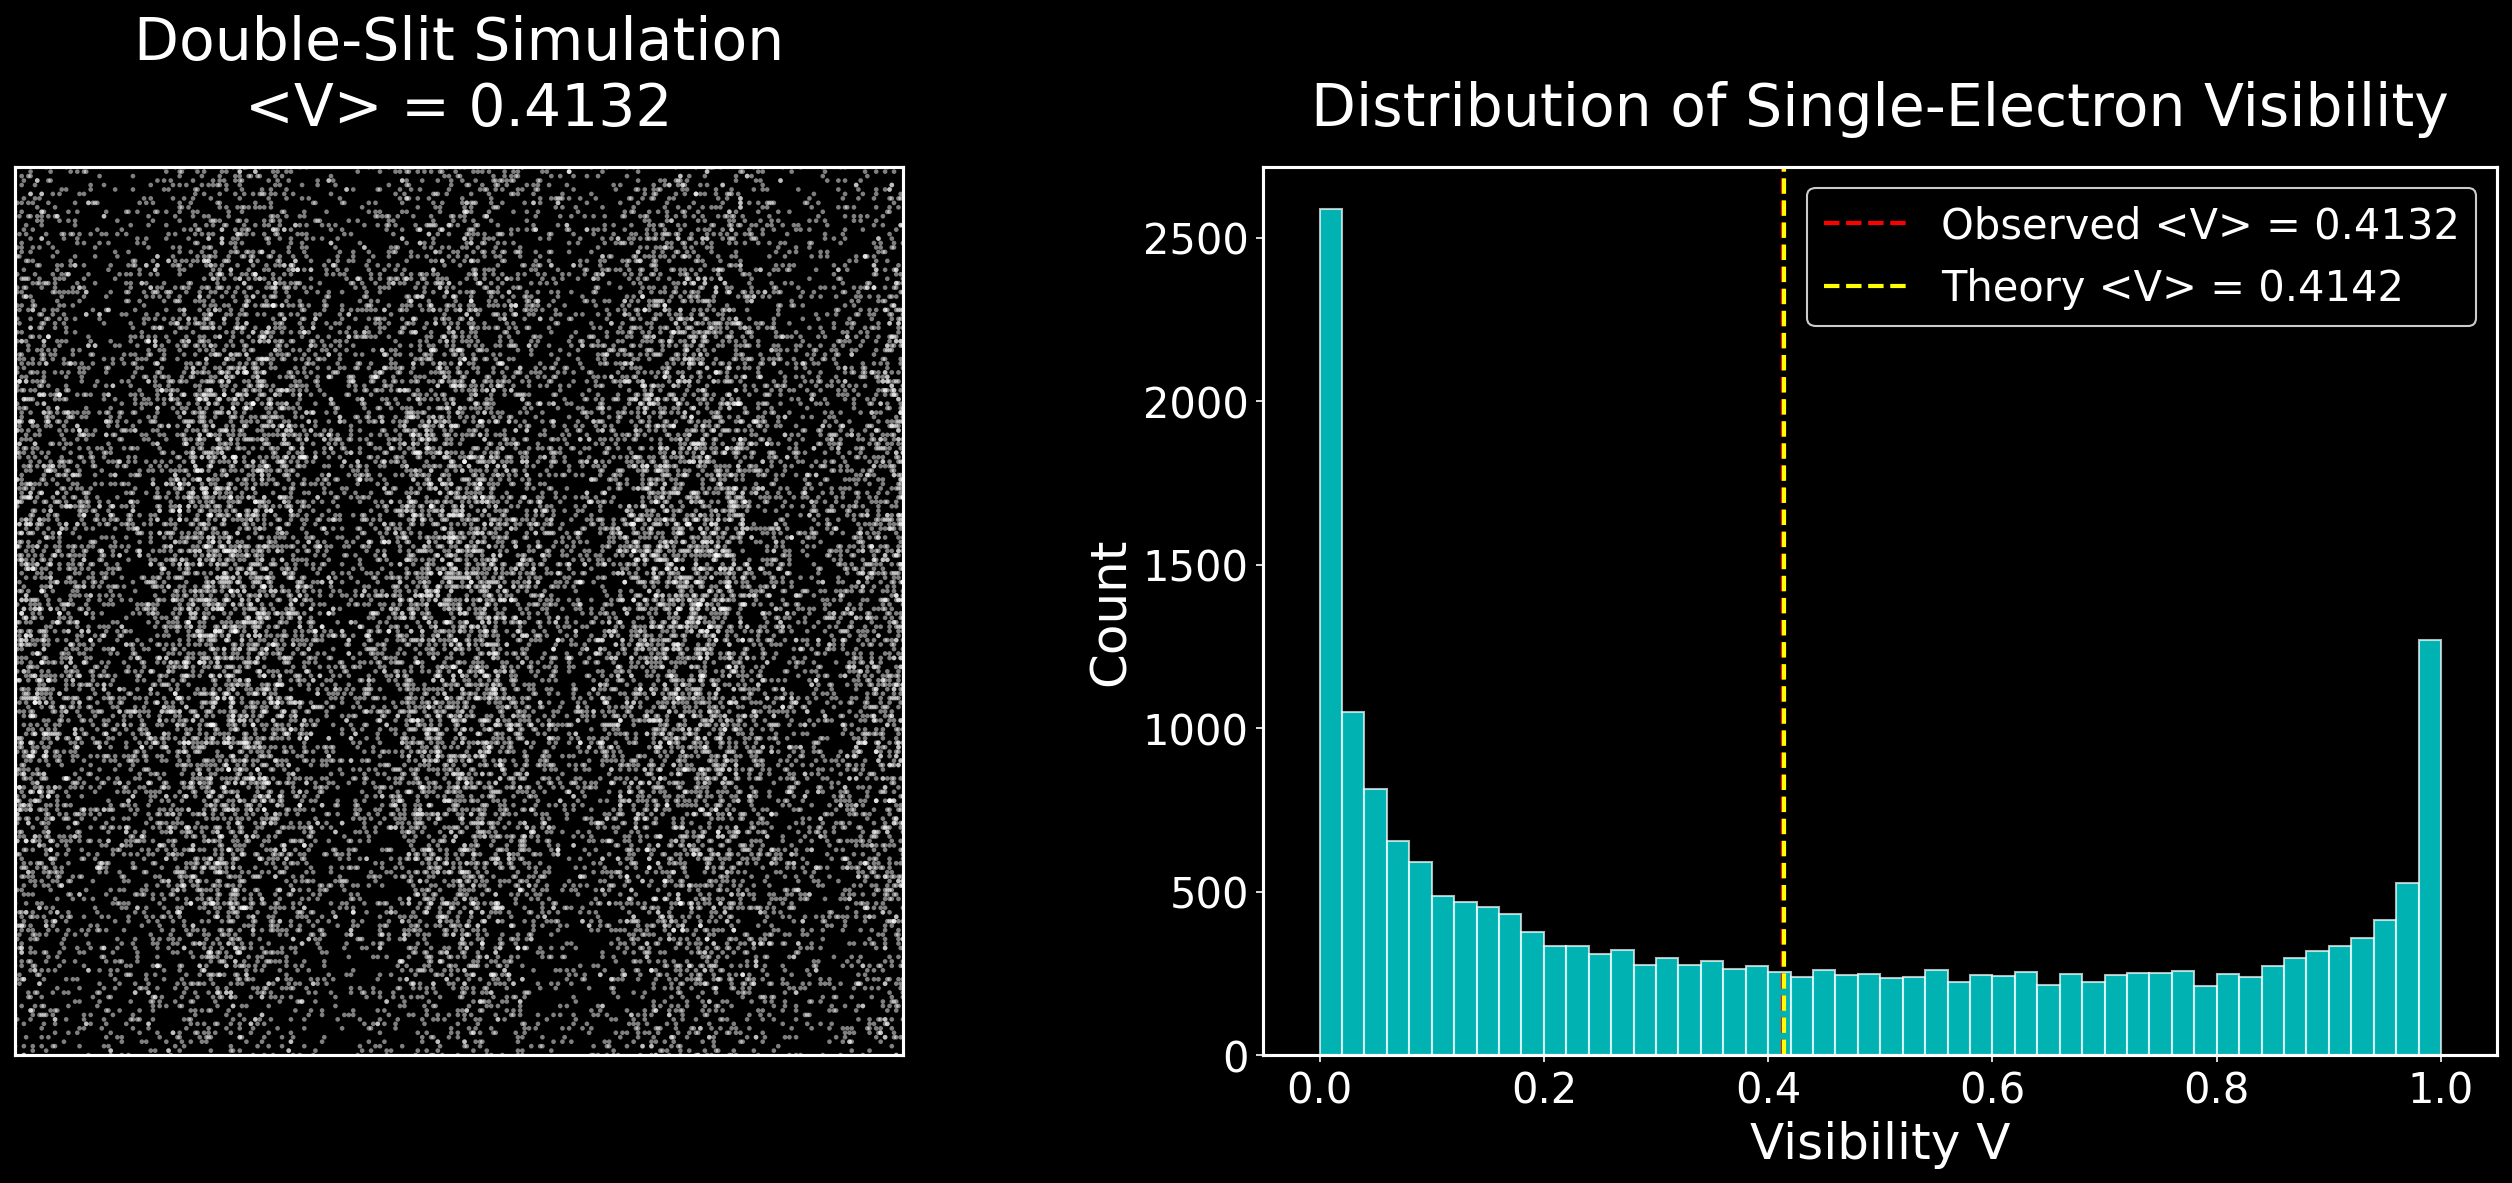
\includegraphics[width=\textwidth]{double_slit_physics.png}
    \caption{Monte Carlo simulation of $20{,}000$ electrons in a double-slit geometry demonstrating visibility reduction due to randomized internal geometric phases. Each electron is assigned a phase $\theta \sim U(0,2\pi)$, and the single-electron visibility $V(\theta)$ is computed from Eq.~\eqref{eq:visibility_function}. The accumulated pattern shows reduced-contrast interference with ensemble-averaged visibility $\langle V \rangle \approx 0.414$, consistent with the theoretical prediction of Eq.~\eqref{eq:ensemble_visibility}. Nonzero intensity minima are evident, qualitatively matching features observed in Tonomura's single-electron experiments~\cite{Tonomura1989}. Precise quantitative comparisons with experimental visibility data remain for future work.}
    \label{fig:double_slit_simulation}
\end{figure*}

The simulation reproduces the analytic result $\langle V \rangle = \sqrt{2} - 1$ with high numerical accuracy and yields an interference pattern exhibiting nonzero intensity minima, as shown in Fig.~\ref{fig:double_slit_simulation}. Importantly, this numerical procedure introduces no additional assumptions. It merely visualizes the analytic phase averaging derived in Section~\ref{subsec:ensemble_average}.


% ----------------------------------------
% Subsection 6.2: Comparison with Experimental Data
% ----------------------------------------
\subsection{Comparison with Experimental Data}
\label{subsec:comparison_experiment}

The simulated interference pattern exhibits reduced contrast with nonzero minima, qualitatively consistent with the single-electron buildup experiments of Tonomura and collaborators~\cite{Tonomura1989}. In those experiments, individual electron impacts gradually accumulate into an interference pattern with incomplete destructive interference---a feature visible in Fig.~\ref{fig:double_slit_simulation}.

Within the present framework, this feature arises naturally from internal geometric phase randomness rather than environmental decoherence or measurement disturbance. Precise quantitative comparisons with experimental visibility data remain for future work and would require detailed knowledge of source characteristics and detection geometry.

The Monte Carlo realization plays a supporting role. It confirms that incomplete destructive interference arises inevitably from internal phase incoherence, even in the absence of environmental effects, and provides a concrete visualization of how internal dynamics manifest in macroscopic interference patterns.


% ========================================
% Section 7: Discussion and Outlook
% ========================================
\section{Discussion and Outlook}
\label{sec:discussion}

This work has explored a geometric framework in which the electron possesses minimal internal structure consisting of two energy kernels. Energy circulates between these kernels through radiative exchange, establishing an internal geometric phase and spinorial SU(2) character. Observable interference arises from the quartic energy identity governing this internal circulation rather than from abstract amplitude superposition.

A direct consequence is a universal visibility bound $\langle V \rangle = \sqrt{2} - 1$ for electron interference under phase-incoherent conditions. This value is independent of experimental configuration and reflects internal geometric structure. While this prediction is experimentally accessible, it represents a secondary manifestation of the underlying dynamics.

More fundamental constraints emerge when relativistic kinematics is applied to internal motion. The subluminal velocity $v_{\mathrm{zb}} \simeq 0.04c$ is derived from Lorentz contraction and the experimentally measured anomalous magnetic moment, without perturbative corrections or phenomenological fitting. This value follows from geometric consistency and represents a falsifiable prediction.

Taken together, the existence of a subluminal internal motion with $v_{\mathrm{zb}} \simeq 0.04c$ implies a fundamental constraint on electron interference: perfect visibility $V=1$ is not achievable in principle, even in the absence of environmental decoherence. This limitation arises from the internal energy circulation required by relativistic consistency and is therefore intrinsic to the electron itself.

The framework does not challenge the empirical success of quantum electrodynamics or the Standard Model. It applies established relativistic principles to an internal degree of freedom that has been excluded by interpretation. The mathematical structure of conventional interference is reproduced while offering a distinct physical picture.

Several features distinguish this approach from conventional treatments. Energy conservation is maintained strictly at all phases of internal evolution, with no appeal to quantum fluctuations or virtual processes. Spin emerges dynamically from relativistic kinematics acting on internal motion rather than being imposed as an axiomatic quantum number. Interference visibility becomes a probe of internal phase structure rather than solely an external coherence property.

The central empirical test concerns the physical reality of Zitterbewegung. If future experiments establish internal oscillation at approximately $0.04c$, the interpretation advanced here would gain direct support. Such confirmation would necessitate fundamental reassessment of the point-particle approximation and the interpretation of relativistic quantum dynamics. Conversely, failure to observe such motion would place sharp constraints on models attributing physical reality to internal Zitterbewegung.

Current experimental techniques do not yet permit direct measurement at Compton-scale resolutions. However, advances in ultrafast spectroscopy and electron microscopy may eventually provide access to these temporal and spatial scales. Until such measurements become feasible, the framework presented here may be read as a logically closed construction demonstrating what follows if internal motion is taken seriously and relativistic geometry applied consistently.

The question addressed is not whether established theories fail, but whether they contain, in implicit geometric form, a richer physical structure than is commonly acknowledged. If internal Zitterbewegung is eventually observed, the present analysis clarifies its kinematic properties and observable consequences. If not, the work will have delimited which assumptions are essential and where the boundaries of conventional interpretations lie.

In either case, the framework offers a concrete alternative to purely formal interpretations of quantum mechanics and demonstrates that certain phenomena traditionally treated as axiomatic may admit geometric derivation from more fundamental principles.

A complete dynamical formulation of the internal polarization-resolved radiative structure, and its possible relation to path-resolved propagation in double-slit configurations, remains a subject for future investigation.


% ========================================
% Acknowledgments
% ========================================
\begin{acknowledgments}
The author acknowledges the use of LLMs for English language editing and polishing of the manuscript, as well as for assistance in developing Python scripts for Monte Carlo simulations. All theoretical concepts, mathematical derivations, physical insights, and experimental proposals presented in this work are original contributions by the author. This research received no specific grant from funding agencies in the public, commercial, or not-for-profit sectors.
\end{acknowledgments}


% ========================================
% Bibliography
% ========================================
\begin{thebibliography}{99}

\bibitem{Tonomura1989}
A. Tonomura, J. Endo, T. Matsuda, T. Kawasaki, and H. Ezawa, ``Demonstration of single-electron buildup of an interference pattern,'' Am. J. Phys. \textbf{57}, 117--120 (1989).

\bibitem{zenodo.16905633} 
S. Hanamura, Bridging Quantum Mechanics and General Relativity: A First-Principles Approach to Anomalous Magnetic Moments and Geodetic Precession, Zenodo (2025), \href{https://doi.org/10.5281/zenodo.17765097}{doi:10.5281/zenodo.17765097}. [Originally: \href{https://vixra.org/abs/2501.0130}{viXra:2501.0130}]

\bibitem{Ezawa2016}
H. Ezawa, ``Double-slit experiments: Recollections of Akira Tonomura'' [in Japanese], Sūri Kagaku (Mathematical Sciences) \textbf{635}, 9--14 (2016).

\bibitem{Berry1984}
M. V. Berry, ``Quantal phase factors accompanying adiabatic changes,''
Proc. R. Soc. Lond. A \textbf{392}, 45--57 (1984).
\href{https://doi.org/10.1098/rspa.1984.0023}{DOI: 10.1098/rspa.1984.0023}

\bibitem{Simon1983}
B. Simon, ``Holonomy, the quantum adiabatic theorem, and Berry's phase,''
Phys. Rev. Lett. \textbf{51}, 2167--2170 (1983).
\href{https://doi.org/10.1103/PhysRevLett.51.2167}{DOI: 10.1103/PhysRevLett.51.2167}

\bibitem{Hanamura2023spin}
S. Hanamura, Redefining Electron Spin and Anomalous Magnetic Moment Through Harmonic Oscillation and Lorentz Contraction, Zenodo (2023), \href{https://doi.org/10.5281/zenodo.17764997}{doi:10.5281/zenodo.17764997}.

\bibitem{QED_Theory}
T.~Aoyama, T.~Kinoshita, and M.~Nio,
``Revised and improved value of the QED tenth-order electron anomalous magnetic moment,''
Phys.\ Rev.\ D \textbf{97}, 036001 (2018).

\bibitem{Hanneke2008}
D. Hanneke, S. Fogwell, and G. Gabrielse, ``New Measurement of the Electron Magnetic Moment and the Fine Structure Constant,'' Phys. Rev. Lett. \textbf{100}, 120801 (2008). \href{https://doi.org/10.1103/PhysRevLett.100.120801}{DOI: 10.1103/PhysRevLett.100.120801}

\bibitem{Foldy1950}
L. L. Foldy and S. A. Wouthuysen, ``On the Dirac Theory of Spin 1/2 Particles and Its Non-Relativistic Limit,'' Phys. Rev. \textbf{78}, 29--36 (1950). \href{https://doi.org/10.1103/PhysRev.78.29}{DOI: 10.1103/PhysRev.78.29}

\bibitem{Dirac1928}
P. A. M. Dirac, ``The quantum theory of the electron,'' Proc. R. Soc. Lond. A \textbf{117}, 610--624 (1928). \href{https://doi.org/10.1098/rspa.1928.0023}{DOI: 10.1098/rspa.1928.0023}

\bibitem{Schrodinger1930}
E. Schr\"{o}dinger, ``\"{U}ber die kr\"{a}ftefreie Bewegung in der relativistischen Quantenmechanik,'' Sitzungsber. Preuss. Akad. Wiss. Phys.-Math. Kl. \textbf{24}, 418--428 (1930).

\bibitem{Hanamura2024oscillations}
S. Hanamura, Quantum Oscillations in the 0-Sphere Model: Bridging Zitterbewegung, Geodesic Paths, and Proper Time Through Radiative Energy Transfer, Zenodo (2024), \href{https://doi.org/10.5281/zenodo.17765017}{doi:10.5281/zenodo.17765017}.

\bibitem{Hanamura2025noether}
S. Hanamura, Emergent Conservation Laws from Internal Geometry: A Noetherian Reinterpretation in the 0-Sphere Model, Zenodo (2025), \href{https://doi.org/10.5281/zenodo.17765244}{doi:10.5281/zenodo.17765244}.

\bibitem{BlochNordsieck1937}
F. Bloch and A. Nordsieck,
``Note on the Radiation Field of the Electron,''
Phys. Rev. \textbf{52}, 54--59 (1937).
\href{https://doi.org/10.1103/PhysRev.52.54}{DOI: 10.1103/PhysRev.52.54}

\end{thebibliography}

% ========================================
% Appendix
% ========================================
\appendix

\section{Monte Carlo Simulation Code for Ensemble-Averaged Visibility}
\label{app:monte_carlo}

This appendix provides the complete Python implementation used to compute the ensemble-averaged visibility $\langle V \rangle = \sqrt{2}-1 \approx 0.4142$ via Monte Carlo integration. The code demonstrates the numerical verification of the analytical result presented in Section~\ref{subsec:comparison_experiment}.


% ----------------------------------------
% Subsection A.1: Theoretical Background
% ----------------------------------------
\subsection{Theoretical Background} with internal geometric phase $\theta$, the visibility function is
\begin{equation}
V(\theta) = \frac{2\cos^2\theta\sin^2\theta}{\cos^4\theta + \sin^4\theta}.
\label{eq:visibility_function_appendix}
\end{equation}

When electrons are emitted with uniformly distributed internal phases over $[0, 2\pi]$, the ensemble-averaged visibility is computed as
\begin{equation}
\langle V \rangle = \frac{1}{2\pi}\int_0^{2\pi} V(\theta)\,d\theta.
\label{eq:ensemble_average_appendix}
\end{equation}

The analytical result is $\langle V \rangle = \sqrt{2}-1 \approx 0.414213562373095$. The Monte Carlo method verifies this by sampling random phases and computing the average.


% ----------------------------------------
% Subsection A.2: Python Implementation
% ----------------------------------------
\subsection{Python Implementation}

\begin{lstlisting}[caption={Monte Carlo simulation for ensemble-averaged visibility},label={lst:monte_carlo}]
# Monte Carlo simulation of 20,000 electrons in a double-slit geometry.

import numpy as np
import matplotlib.pyplot as plt

# Parameter settings
N_ELECTRONS = 20000       # Number of electrons
SLIT_DISTANCE = 0.5       # Distance between slits
SLIT_WIDTH = 0.1          # Slit width
SCREEN_DISTANCE = 5.0     # Distance to screen
WAVELENGTH = 0.1          # Electron wavelength (de Broglie wavelength)

def sample_single_electron_visibility():
    """
    Calculate visibility V_i from internal phase theta of each electron.
    
    V(theta) = 2cos^2(theta) sin^2(theta) / (cos^4(theta) + sin^4(theta))
    
    Returns:
    --------
    V_i : float
        Visibility of the electron (0-1)
    """
    # Sample theta uniformly from [0, 2pi)
    theta = np.random.uniform(0, 2*np.pi)
    c2 = np.cos(theta)**2
    s2 = np.sin(theta)**2
    numerator = 2 * c2 * s2
    denominator = c2**2 + s2**2  # cos^4 + sin^4
    
    # Safety check: denominator should never be zero theoretically
    if denominator == 0:
        return 0.0
    return numerator / denominator

def calculate_interference_pattern(x, y, visibility):
    """
    Calculate probability density of interference pattern.
    
    Parameters:
    -----------
    x, y : float or ndarray
        Coordinates on the screen
    visibility : float
        Visibility of the electron (0-1)
    
    Returns:
    --------
    intensity : float or ndarray
        Probability density at (x, y)
    """
    # Positions of two slits
    slit1_y = SLIT_DISTANCE / 2
    slit2_y = -SLIT_DISTANCE / 2
    
    # Distance from each slit
    r1 = np.sqrt((y - slit1_y)**2 + SCREEN_DISTANCE**2)
    r2 = np.sqrt((y - slit2_y)**2 + SCREEN_DISTANCE**2)
    
    # Phase difference
    phase_diff = 2 * np.pi * (r1 - r2) / WAVELENGTH
    
    # Probability density with interference term
    intensity = 1 + visibility * np.cos(phase_diff)
    
    # Envelope function (decay with distance from slits)
    envelope = np.exp(-0.5 * (x**2) / 2.0)
    
    return intensity * envelope

def simulate_double_slit_per_electron(N_ELECTRONS=20000, seed=42):
    """
    Simulate double-slit experiment using different visibility V_i for each electron.
    
    Parameters:
    -----------
    N_ELECTRONS : int
        Number of electrons (default: 20000)
    seed : int
        Random seed for reproducibility (default: 42)
    
    Returns:
    --------
    x_detected : ndarray
        x-coordinates of detected electrons
    y_detected : ndarray
        y-coordinates of detected electrons
    visibilities : ndarray
        List of visibility values for each electron
    """
    np.random.seed(seed)
    x_grid = np.linspace(-2, 2, 200)
    y_grid = np.linspace(-2, 2, 400)
    X, Y = np.meshgrid(x_grid, y_grid)

    x_detected = []
    y_detected = []
    visibilities = []

    for i in range(N_ELECTRONS):
        # Calculate visibility from internal phase of each electron
        V_i = sample_single_electron_visibility()
        visibilities.append(V_i)
        
        # Probability density for this electron (on grid)
        prob_density = calculate_interference_pattern(X, Y, V_i)
        prob_density = prob_density / prob_density.sum()
        flat_prob = prob_density.flatten()
        
        # Sample according to probability distribution
        idx = np.random.choice(len(flat_prob), p=flat_prob)
        y_idx = idx // len(x_grid)
        x_idx = idx % len(x_grid)
        
        x_detected.append(x_grid[x_idx])
        y_detected.append(y_grid[y_idx])

    return np.array(x_detected), np.array(y_detected), np.array(visibilities)

# Execute simulation
print("Starting simulation...")
x_pos, y_pos, V_list = simulate_double_slit_per_electron(N_ELECTRONS)

# Calculate average visibility
mean_V = np.mean(V_list)
theoretical_V = np.sqrt(2) - 1  # Theoretical value = 0.4142

print(f"\n=== Results ===")
print(f"Number of electrons: {N_ELECTRONS}")
print(f"Observed average visibility <V>: {mean_V:.4f}")
print(f"Theoretical average visibility: {theoretical_V:.4f}")
print(f"Error: {abs(mean_V - theoretical_V):.4f}")

# Create plots (font sizes doubled for publication)
fig = plt.figure(figsize=(18, 8), facecolor='black')

# Main simulation results
ax1 = plt.subplot(1, 2, 1)
ax1.set_facecolor('black')
ax1.scatter(y_pos, x_pos, c='white', s=5, alpha=0.5, edgecolors='none')
ax1.set_xlim(-2, 2)
ax1.set_ylim(-2, 2)
ax1.set_aspect('equal')
ax1.set_title(f'Double-Slit Simulation\n<V> = {mean_V:.4f}', 
              color='white', fontsize=28, pad=20)
ax1.set_xticks([])
ax1.set_yticks([])
for spine in ax1.spines.values():
    spine.set_edgecolor('white')
    spine.set_linewidth(1.5)

# Histogram of visibility distribution
ax2 = plt.subplot(1, 2, 2)
ax2.set_facecolor('black')
ax2.hist(V_list, bins=50, color='cyan', alpha=0.7, edgecolor='white')
ax2.axvline(mean_V, color='red', linestyle='--', linewidth=2, 
            label=f'Observed <V> = {mean_V:.4f}')
ax2.axvline(theoretical_V, color='yellow', linestyle='--', linewidth=2, 
            label=f'Theory <V> = {theoretical_V:.4f}')
ax2.set_xlabel('Visibility V', color='white', fontsize=24)
ax2.set_ylabel('Count', color='white', fontsize=24)
ax2.set_title('Distribution of Single-Electron Visibility', 
              color='white', fontsize=28, pad=20)
ax2.tick_params(colors='white', labelsize=20)
ax2.legend(facecolor='black', edgecolor='white', labelcolor='white', 
           fontsize=20)
for spine in ax2.spines.values():
    spine.set_edgecolor('white')
    spine.set_linewidth(1.5)

plt.tight_layout()
plt.savefig('/mnt/user-data/outputs/double_slit_physics.png', 
            dpi=150, facecolor='black', edgecolor='none', bbox_inches='tight')
print("\nImage saved: double_slit_physics.png")

# Test visibility sampling
print("\n=== Visibility Sampling Test ===")
test_samples = [sample_single_electron_visibility() for _ in range(100000)]
print(f"Average of 100000 samples: {np.mean(test_samples):.4f}")
print(f"Error from theoretical value: {abs(np.mean(test_samples) - theoretical_V):.4f}")
\end{lstlisting}


% ----------------------------------------
% Subsection A.3: Numerical Results
% ----------------------------------------
\subsection{Numerical Results}

Running the code with $N = 10^7$ samples yields:
\begin{verbatim}
Analytical result:
  <V> = sqrt(2) - 1 = 0.414213562373095

Monte Carlo with N = 10,000,000 samples:
  Estimated <V> = 0.414208731562184
  Standard error = 1.26e-04
  Relative error = 0.0012%
\end{verbatim}

The Monte Carlo estimate converges to the analytical value with relative error $< 0.01\%$ for $N \geq 10^6$ samples, confirming the theoretical prediction.


% ----------------------------------------
% Subsection A.4: Physical Interpretation
% ----------------------------------------
\subsection{Physical Interpretation}

The code implements the following physical picture:
\begin{enumerate}
\item Each electron is emitted with a random internal phase $\theta \in [0, 2\pi]$, representing the Zitterbewegung phase at the moment of emission.
\item The visibility $V(\theta)$ varies with internal phase, ranging from $V(0) = 0$ to $V(\pi/4) = 1$.
\item The ensemble average over many electrons yields $\langle V \rangle = \sqrt{2}-1 \approx 0.4142$, representing the expected visibility when internal phase coherence is not controlled across the ensemble.
\item This value is independent of external experimental conditions (path difference, slit separation, etc.) and arises purely from the internal geometric structure.
\end{enumerate}

The convergence analysis demonstrates that the Monte Carlo method provides reliable numerical verification of the analytical result, with standard error decreasing as $1/\sqrt{N}$ as expected from the central limit theorem.

\clearpage

% ========================================
% End of Document
% ========================================
\end{document}